\documentclass[twoside,12pt]{article}
\usepackage{amssymb,amsmath, amsfonts,latexsym,mathtext, array, graphicx, geometry, caption, subcaption, bbm}
\geometry{margin=1.5cm}
\setlength{\parskip}{0.8ex plus 0.1ex minus 0.2ex}
\newcommand{\M}[1]{\boldsymbol{\mathbf{#1}}}
\newcommand{\V}{\M}
\newcommand{\Cal}{\mathcal}
\bibliographystyle{plain}

\newtheorem{thm1}{Theorem}
\newtheorem{def1}{Definition}

\begin{document}

\title{Machine Learning 6.867 - Final Report\\Robust Artificial Neural Networks}
\author{Ying (Daisy) Zhuo}

\maketitle

Artificial neural networks (ANN) have been shown to have very strong performance for many challenging machine learning tasks such as image recognition and natural language processing. This is largely due to its ability to approximate non-linear functions arbitrarily well and to extract patterns from complicated or noisy data. However, the generalization performance of neural networks can be severely impacted by overfitting the training set. This project presents a Robust-ANN formulation and demonstrates the benefits it offers. 

\section{Introduction}

Regularization is classical approach to reduce overfitting in many machine learning methods. By adding a penalty on the weight parameters to the objective function, the weight parameters are shrunk toward zero. Smaller weights give smoother network response and can potentially reduce overfit. One simple regularizer is \emph{weight decay}, which adds a $\lambda \M w ^T \M w$ term to the error function. In a probabilistic view, simple weight decay regularization is equivalent to putting a Gaussian prior over the weight parameters. 

Unfortunately, simple weight decay does not achieve the desirable property of \emph{consistency}, also known as scaling invariance. The invariance property says if we linearly transform the input or target vector, we should obtain equivalent network with linear transformation of weights as given. However, the simple weight decay regularizer term does not maintain this property, as it penalizes on all weights equally. One scale-invariant regularizer is to use different trade-off parameters for the two weights; i.e., adding $\lambda_1 \| \M w^{(1)}\|^2 + \lambda_2 \| \M w^{(2)}\|^2$ to the negative log likelihood, biases excluded. In the Bayesian framework, putting different priors on $\M w^{(1)}$ and $\M w^{(2)}$ corresponds to an improper prior, which cannot be normalized. Using improper priors can lead to difficulty in selecting regularization coefficients and Bayesian model comparisons. 

In this project, I would like to explore the feasibility of robustifying neural networks. My hypothesis is that it is possible, and can be shown to resemble regularization under specific choice of uncertainty sets. Since robust methods inherently consider data being altered, it should not have issue with scaling invariance as simple weight decay does. I will discuss the computational tractability of robust neural networks. Further, I will test it on multiple datasets. My research group has collected 70+ datasets from UCI Machine Learning Repository with classification tasks, and I plan to test the magnitude of improvements on a sizable subset.

Many other practical approaches to improve neural networks exist. One method is to artificially expand the training data, knowing that the model should be invariant to translation and scaling. 

\section{Overview of Robust Optimization}
Given the somewhat ad hoc nature of adding regularizers and difficulty in the Bayesian framework on neural networks, I would like to consider the issue from a different perspective. In a recent paper, Bertsimas et al. proposed a principled approach using Robust Optimization to model data uncertainty, and have shown its equivalence to regularization in certain circumstances \cite{bertsimas2015robust}. For example, by modeling uncertainty in input features  on hinge-loss minimization, it is equivalent to support vector machines. The computational results in the paper suggest that systematically addressing uncertainties generalizes better than regularization, as demonstrated in logistic regression, support vector machine, and decision trees. 



We give an overview of robust optimization and introduce the notions of uncertainty sets and dual norms that will be used later when applying robust optimization techniques to artificial neural networks. some of the content below is adapted from \cite{bertsimas2015robust}.

Robust optimization is a means for modeling uncertainty in optimization problems without the use of probability distributions.
Under this modeling framework, we construct deterministic \emph{uncertainty sets} that contain possible values of uncertain parameters. We then seek a solution that is optimal for all such realizations of this uncertainty. Consider the general optimization problem:
\[
\begin{aligned}
  \max_{\V x \in \Cal X} ~~ & c(\V u, \V x)\\
  \textup{s.t.} ~~ & \V g (\V u, \V x) \le 0.
\end{aligned}
\]
where $\V x$ is the vector of decision variables, and $\V u$ is a vector of given parameters. Relaxing the assumption that $\V u$ is fixed, we assume instead that the realized values of $\V u$ are restricted to be within some uncertainty set $\Cal U$. We form the corresponding robust optimization problem by optimizing against the worst-case realization of the uncertain parameters across the entire uncertainty set:
\[
\begin{aligned}
  \max_{\V x \in \Cal X} ~~ & \min_{\V u \in \Cal U} \; c(\V u, \V x) \\
  \textup{s.t.} ~~ & \V g (\V u, \V x) \le 0 ~~ \forall \V u \in \Cal U.
\end{aligned}
\]
Despite typically having an infinite number of constraints, it is often possible to reformulate the problem as a deterministic optimization problem with finite size, depending on the choice of uncertainty set $\Cal U$. The resulting deterministic problem is deemed the \emph{robust counterpart}, which is generally a problem of the same complexity as the nominal problem.

There is extensive evidence in the literature that robust solutions have significant advantages relative to nominal solutions.


\section{Theoretical Derivation}

connection to regularization?

\section{Implementation and Computational Results}
I implemented Robust-ANN in the programming language \textsf{Julia} with package \textsf{MXNet}, an efficient and flexible deep learning framework \cite{mxnet}. To benchmark, the implementation is tested on the MNIST dataset of handwritten digits, with $50,000$ data points in training, $10,000$ in evaluation, each of dimension $784$. The outputs are digits $0$ through $9$. The network structure has three layers and is presented in Figure~\ref{fig:ann_arc}. Other model specifications include: number of epoch is 3 to ensure baseline method obtains decent accuracy, learning rate is 0.1, momentum is 0.9, weight decay coefficient is 0.00001. We use a stochastic gradient descent optimizer, with batch size being 100. Since the problem size is small, we only use CPU for this purpose. 
\begin{figure}[ht!]
    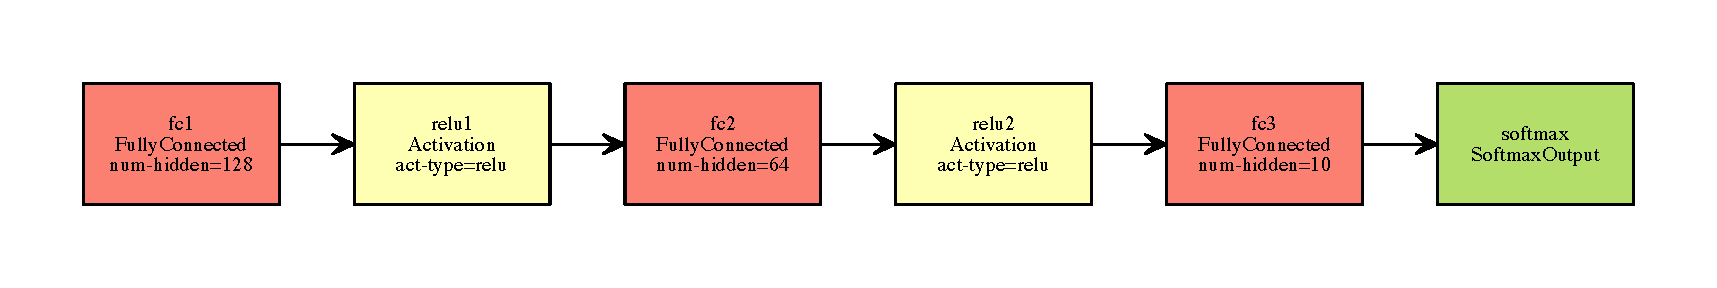
\includegraphics[scale=0.7]{visualize.pdf}
    \caption{Illustration of ANN architecture in computational tests.}
    \label{fig:ann_arc}
\end{figure}



The procedure in Robust-ANN is as follows: after an iteration of normal ANN, a backward call is ran on each small batch to obtain the gradients. A small complication is that \textsf{MXNet} does not provide gradient with respect to the data $\M x_i$, we take the current first level weights $\M w$, the gradient with respect to the ReLU activation $\frac{\partial J}{\partial \M a}$ and do the following calculation:


\begin{equation}
\begin{aligned}
\frac{\partial J}{\partial \M x} 
& = \sum_{j=1}^{n_1} \frac{\partial J}{\partial a_j} h'(\M w_j^T \M x) \M w_j\\
& = \sum_{j=1}^{n_1} \frac{\partial J}{\partial a_j} \mathbbm{1}_{\{\M w_j^T \M x > 0 \} } \M w_j
\end{aligned}
\end{equation}

Depending on the choice of uncertainty set, we can construct the adversarial $\Delta \M x_i$ differently. In this example, we consider the $l_\infty$ norm uncertainty set and therefore obtain $\M x_i^{\textrm{new}} = \M x_i^{\textrm{old}} + \rho * sign(\frac{\partial J}{\partial \M x})$.

\section{Conclusions}



\bibliography{ref}

\end{document}